\documentclass[../../labo_tp5_main.tex]{subfiles}

\begin{document}

%capítulo
\section{Ejercicio 3}

La modulación AM (Amplitude Modulation) consiste en modificar la amplitud de una señal portadora senoidal, $S_p(t)$ de amplitud y frecuencia fija, en base a la amplitud de una señal moduladora, $S_m(t)$. 
La señal modulada por AM estará dada entonces por la fórmula $S_{AM}(t) = (1 + m\cdot S_m(t))\cdot S_p(t)$, donde m es el coeficiente de modulación, definido por: $\frac{V_{max} - V_{min}}{V_{max} + V_{min}}$.\par
Observando la modulación entre señales senoidales, podremos luego analizar el caso en que $S_m(t)$ no sea senoidal por superposición. \par

Para el caso en que tanto $S_p(t)$ como $S_m(t)$ sean senoidales, por lo tanto, se obtendrá:\par
\begin{center}
$S_{AM}(t) = A_p\cdot (1 + m\cdot cos(2\pi f_m\cdot\cdot t))\cdot cos(2\pi f_p\cdot t)$\par
$S_{AM}(t) = A_p\cdot cos(2\pi f_p\cdot t) + A_p\cdot cos(2\pi f_p\cdot t)\cdot m\cdot cos(2\pi f_m\cdot\cdot t)\cdot cos(2\pi f_p\cdot t)$\par
$S_{AM}(t) = A_p\cdot cos(2\pi f_p\cdot t) + \frac{A_p\cdot m}{2}\cdot [cos(2\pi \cdot (f_p-f_m)\cdot t) + cos(2\pi (f_p+f_m)\cdot t)]$\par
\end{center}

Por lo que se observarán tres frecuencias principales para la señal modulada y luego sus respectivos armónicos.\par
Por consigna, se deberá modular con AM una señal portadora de 1.9MHz y una moduladora de 100kHz. Por límites de frecuencia, se tuvo que usar dos generadores distintos para poder modular externamente.\par
La señal modulada era de $200mV_{pp}$ 

Se muestran los espectros simulados en conjunto con los obtenidos por medición:

\begin{figure}[H]	
	\centering
	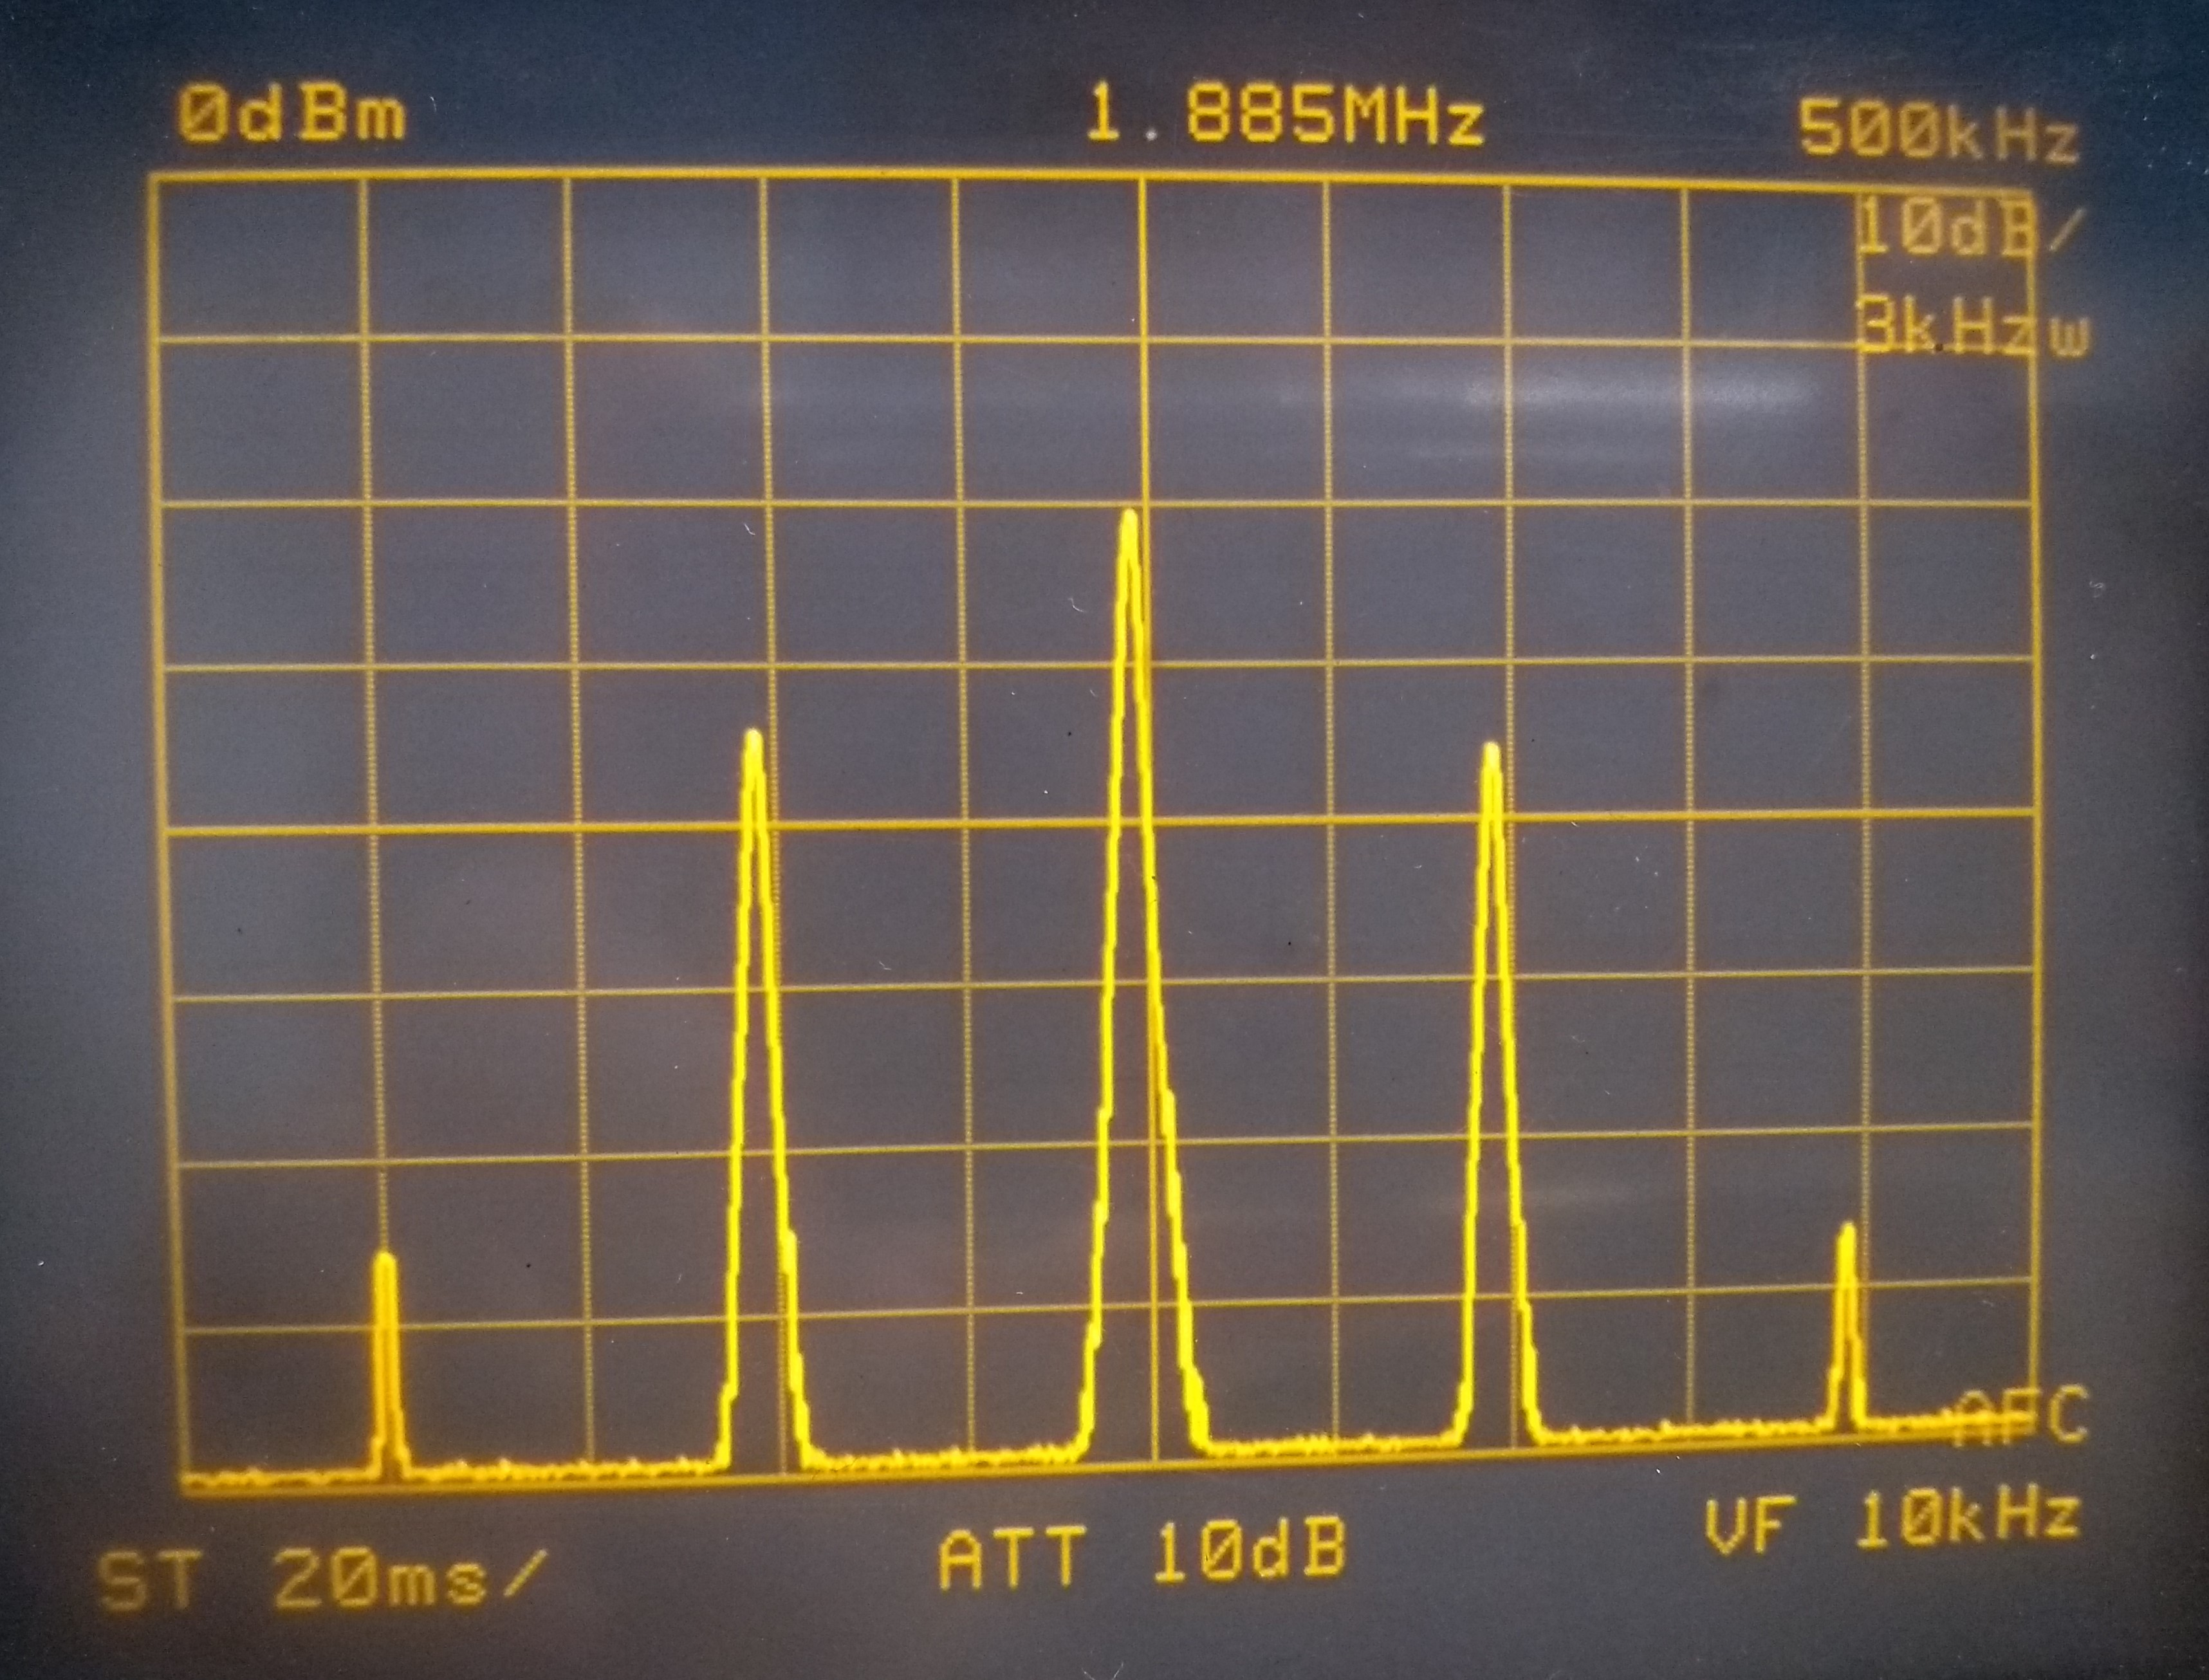
\includegraphics[scale=0.05]{imagenes/labo_tp5_ej3_a_1.jpg}
	\caption{Mediciones del espectro de una señal moduladora senoidal con m=0.5}
	\label{fig:ej1_labo_tp5_ej3_a_1}
\end{figure}
\begin{figure}[H]	
	\centering
	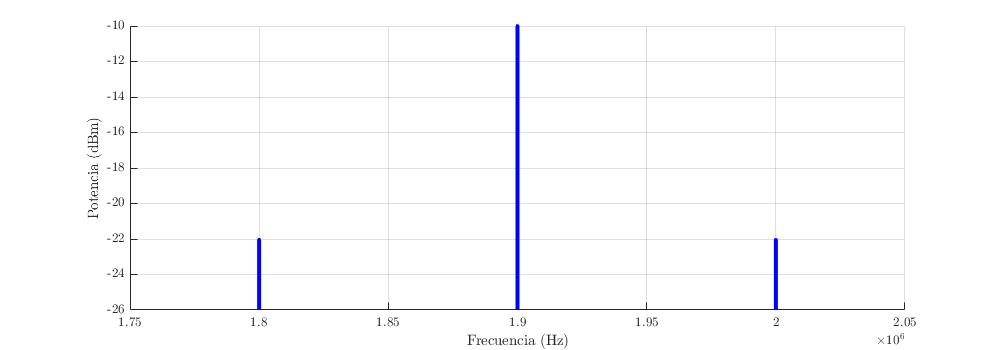
\includegraphics[scale=0.5]{imagenes/labo_tp5_ej3a.jpg}
	\caption{Mediciones del espectro de una señal moduladora senoidal con m=0.5}
	\label{fig:ej1_labo_tp5_ej3_a_1}
\end{figure}
\begin{figure}[H]	
	\centering
	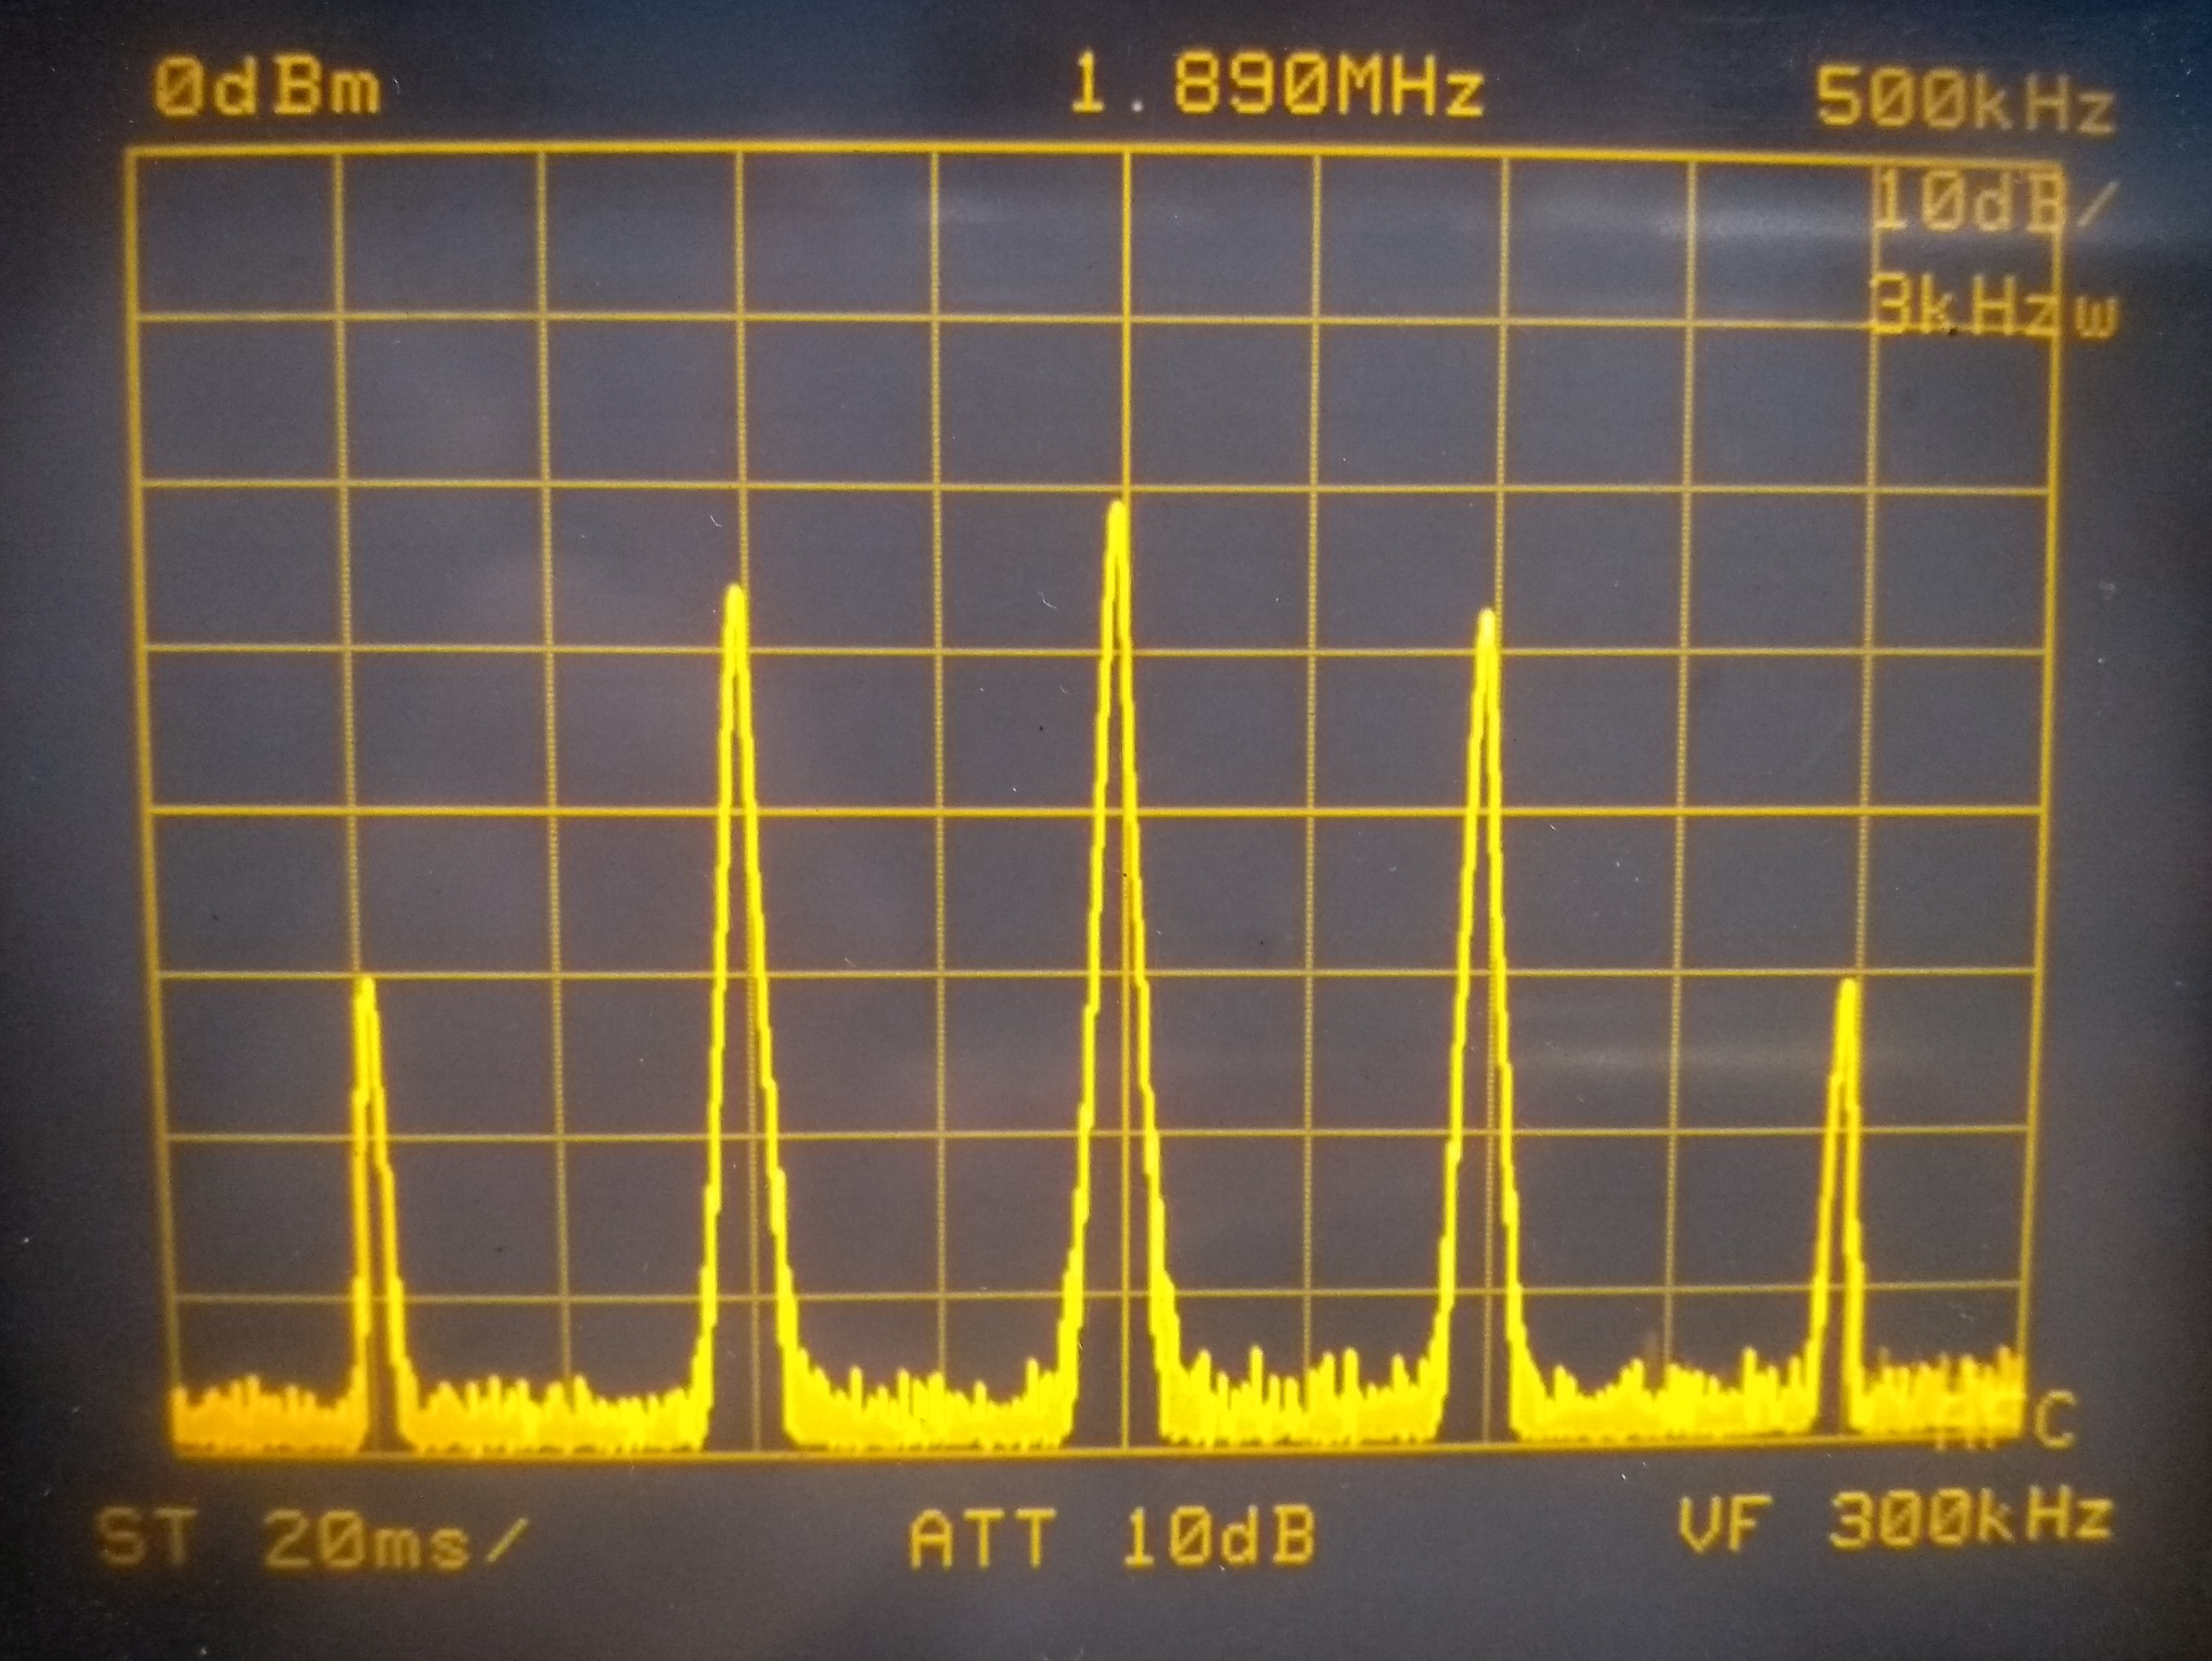
\includegraphics[scale=0.05]{imagenes/labo_tp5_ej3_b.jpg}
	\caption{Mediciones del espectro de una señal moduladora senoidal con m=1}
	\label{fig:ej1_labo_tp5_ej3_b}
\end{figure}
\begin{figure}[H]	
	\centering
	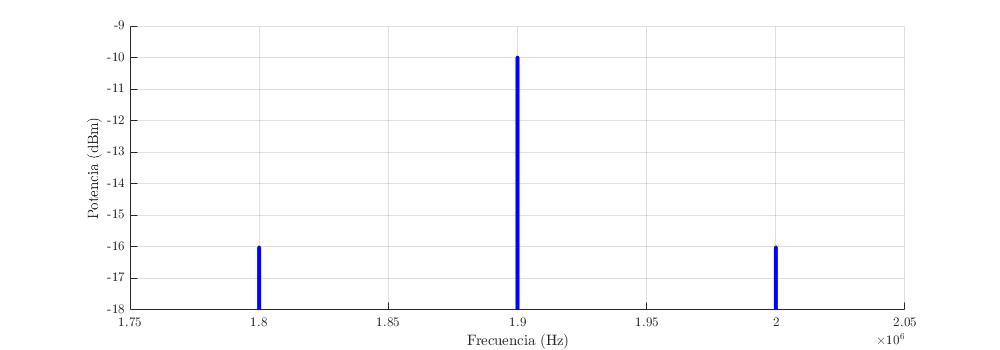
\includegraphics[scale=0.5]{imagenes/labo_tp5_ej3b.jpg}
	\caption{Simulaciones del espectro de una señal moduladora senoidal con m=1}
	\label{fig:ej1_labo_tp5_ej3_b}
\end{figure}
\begin{figure}[H]	
	\centering
	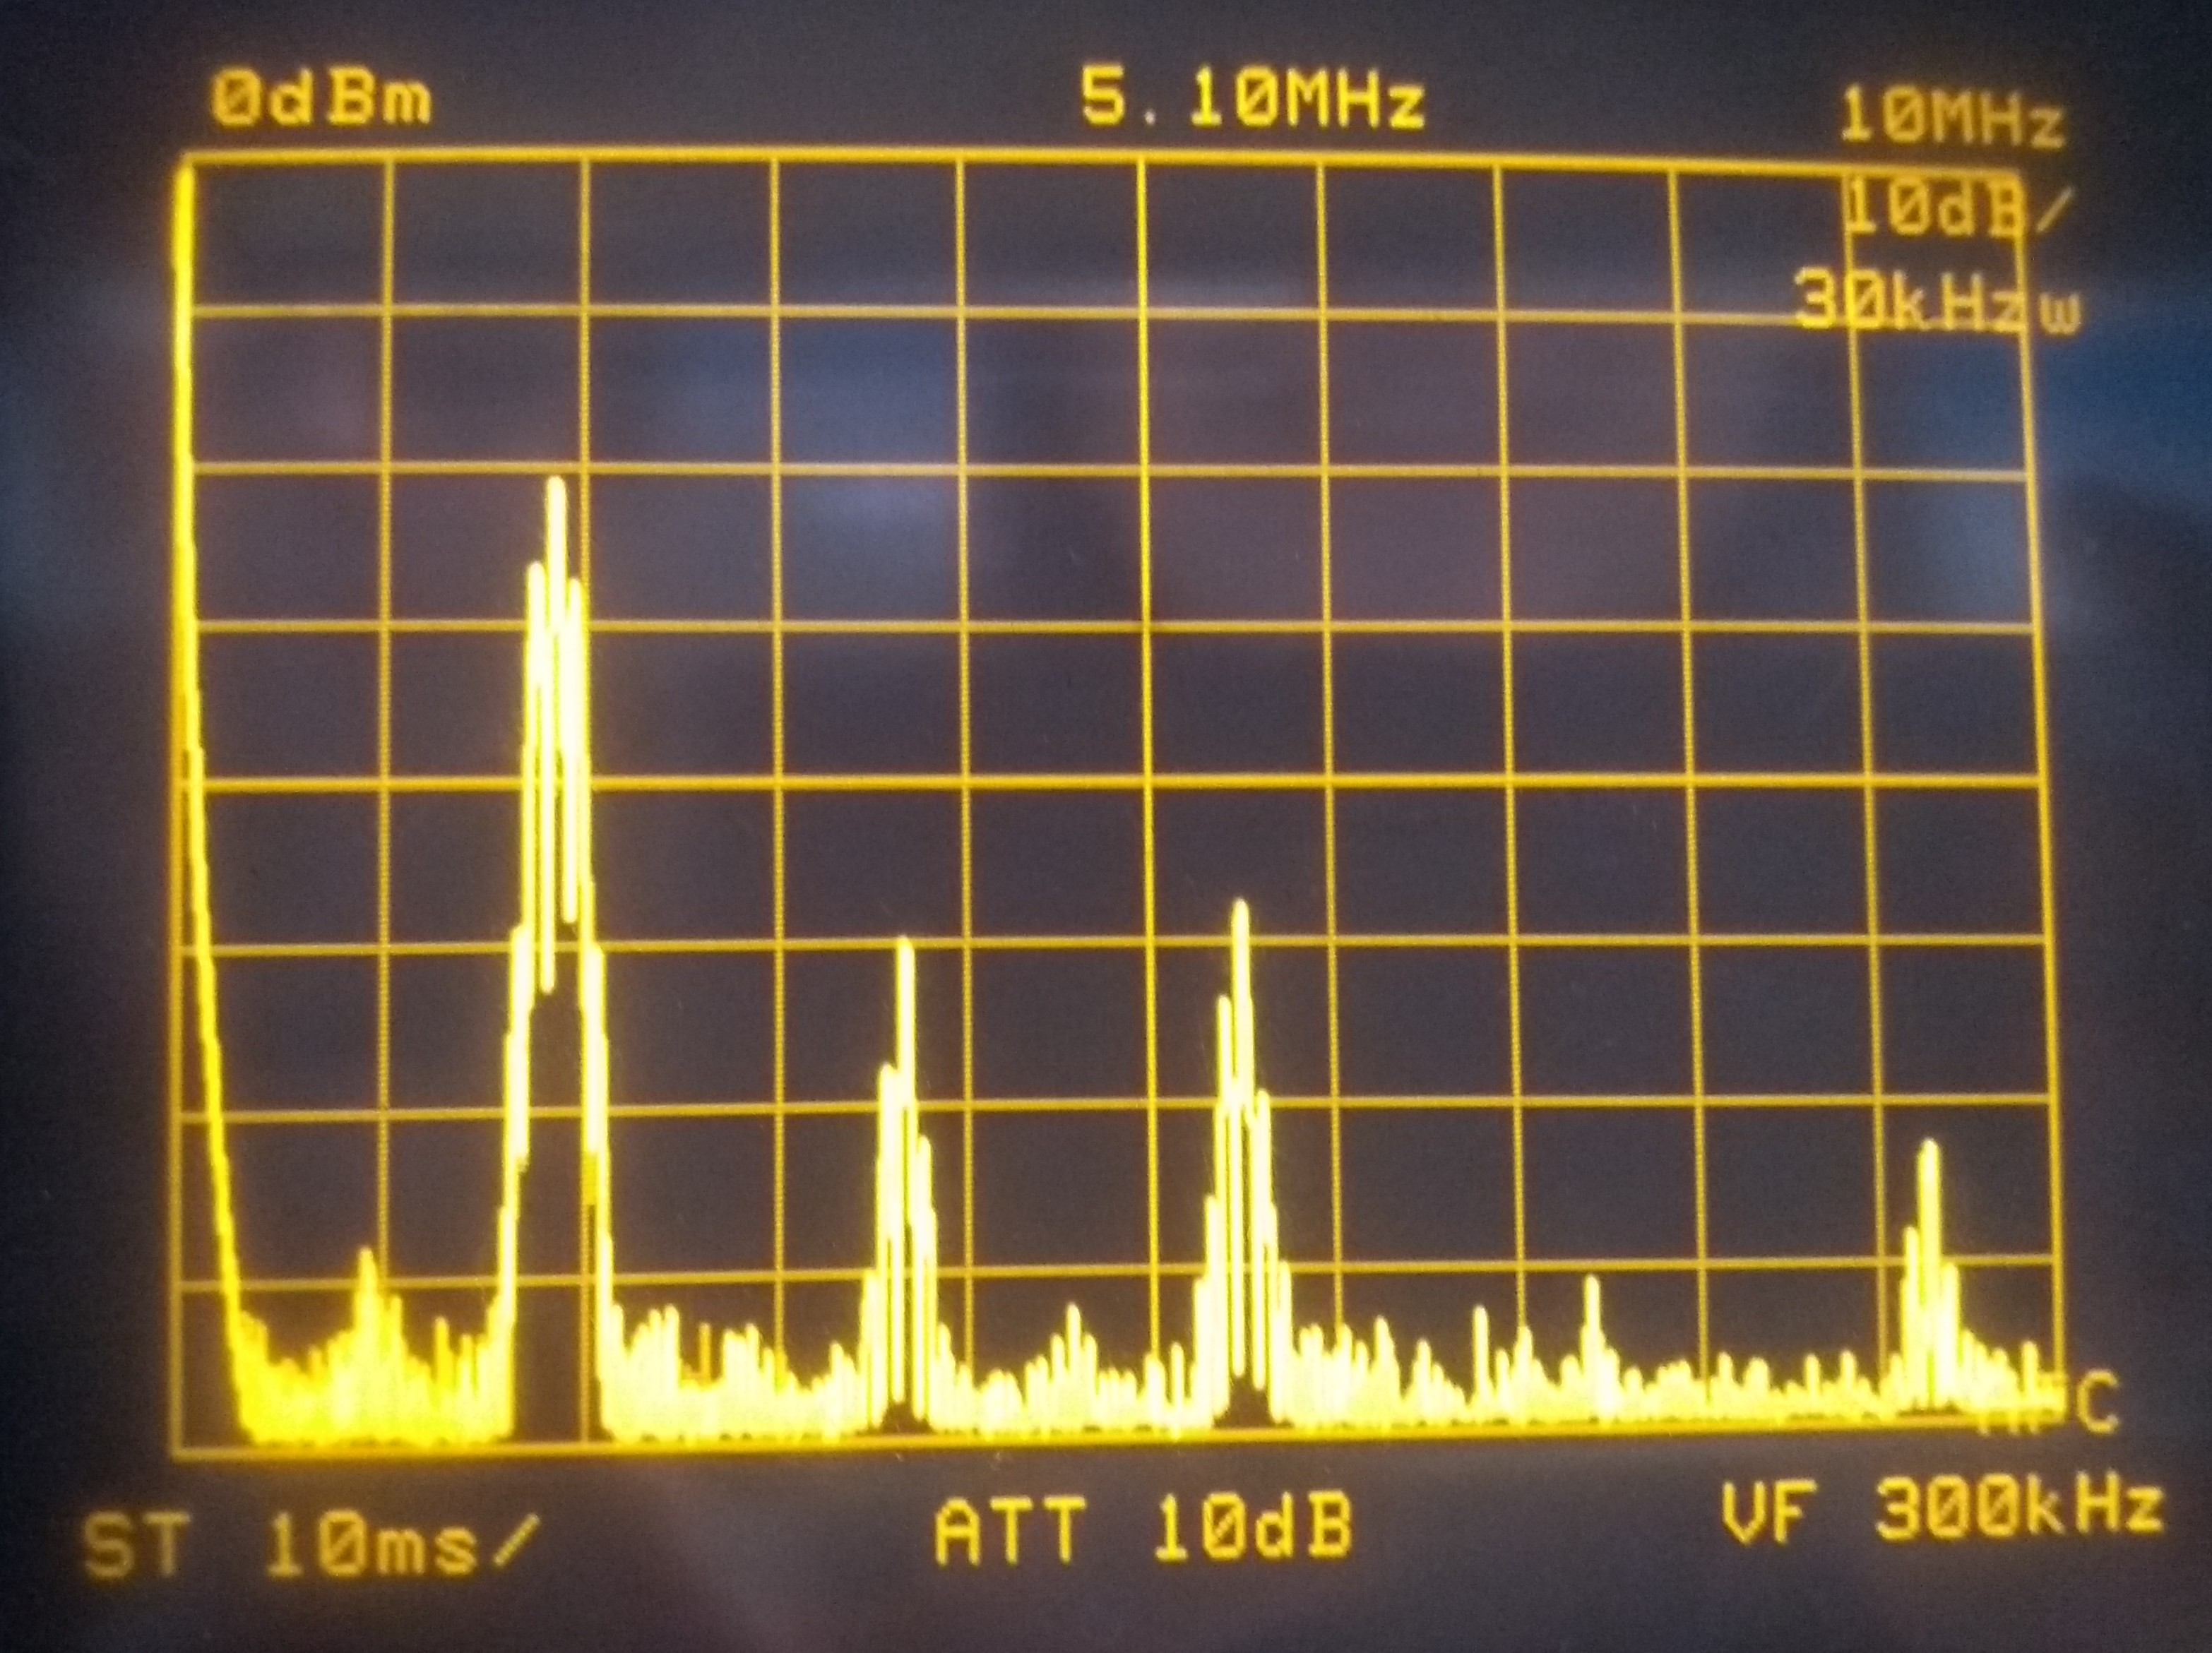
\includegraphics[scale=0.05]{imagenes/labo_tp5_ej3_b_2.jpg}
	\caption{Mediciones del espectro de una señal moduladora senoidal con m=1}
	\label{fig:ej1_labo_tp5_ej3_b_2}
\end{figure}
\begin{figure}[H]	
	\centering
	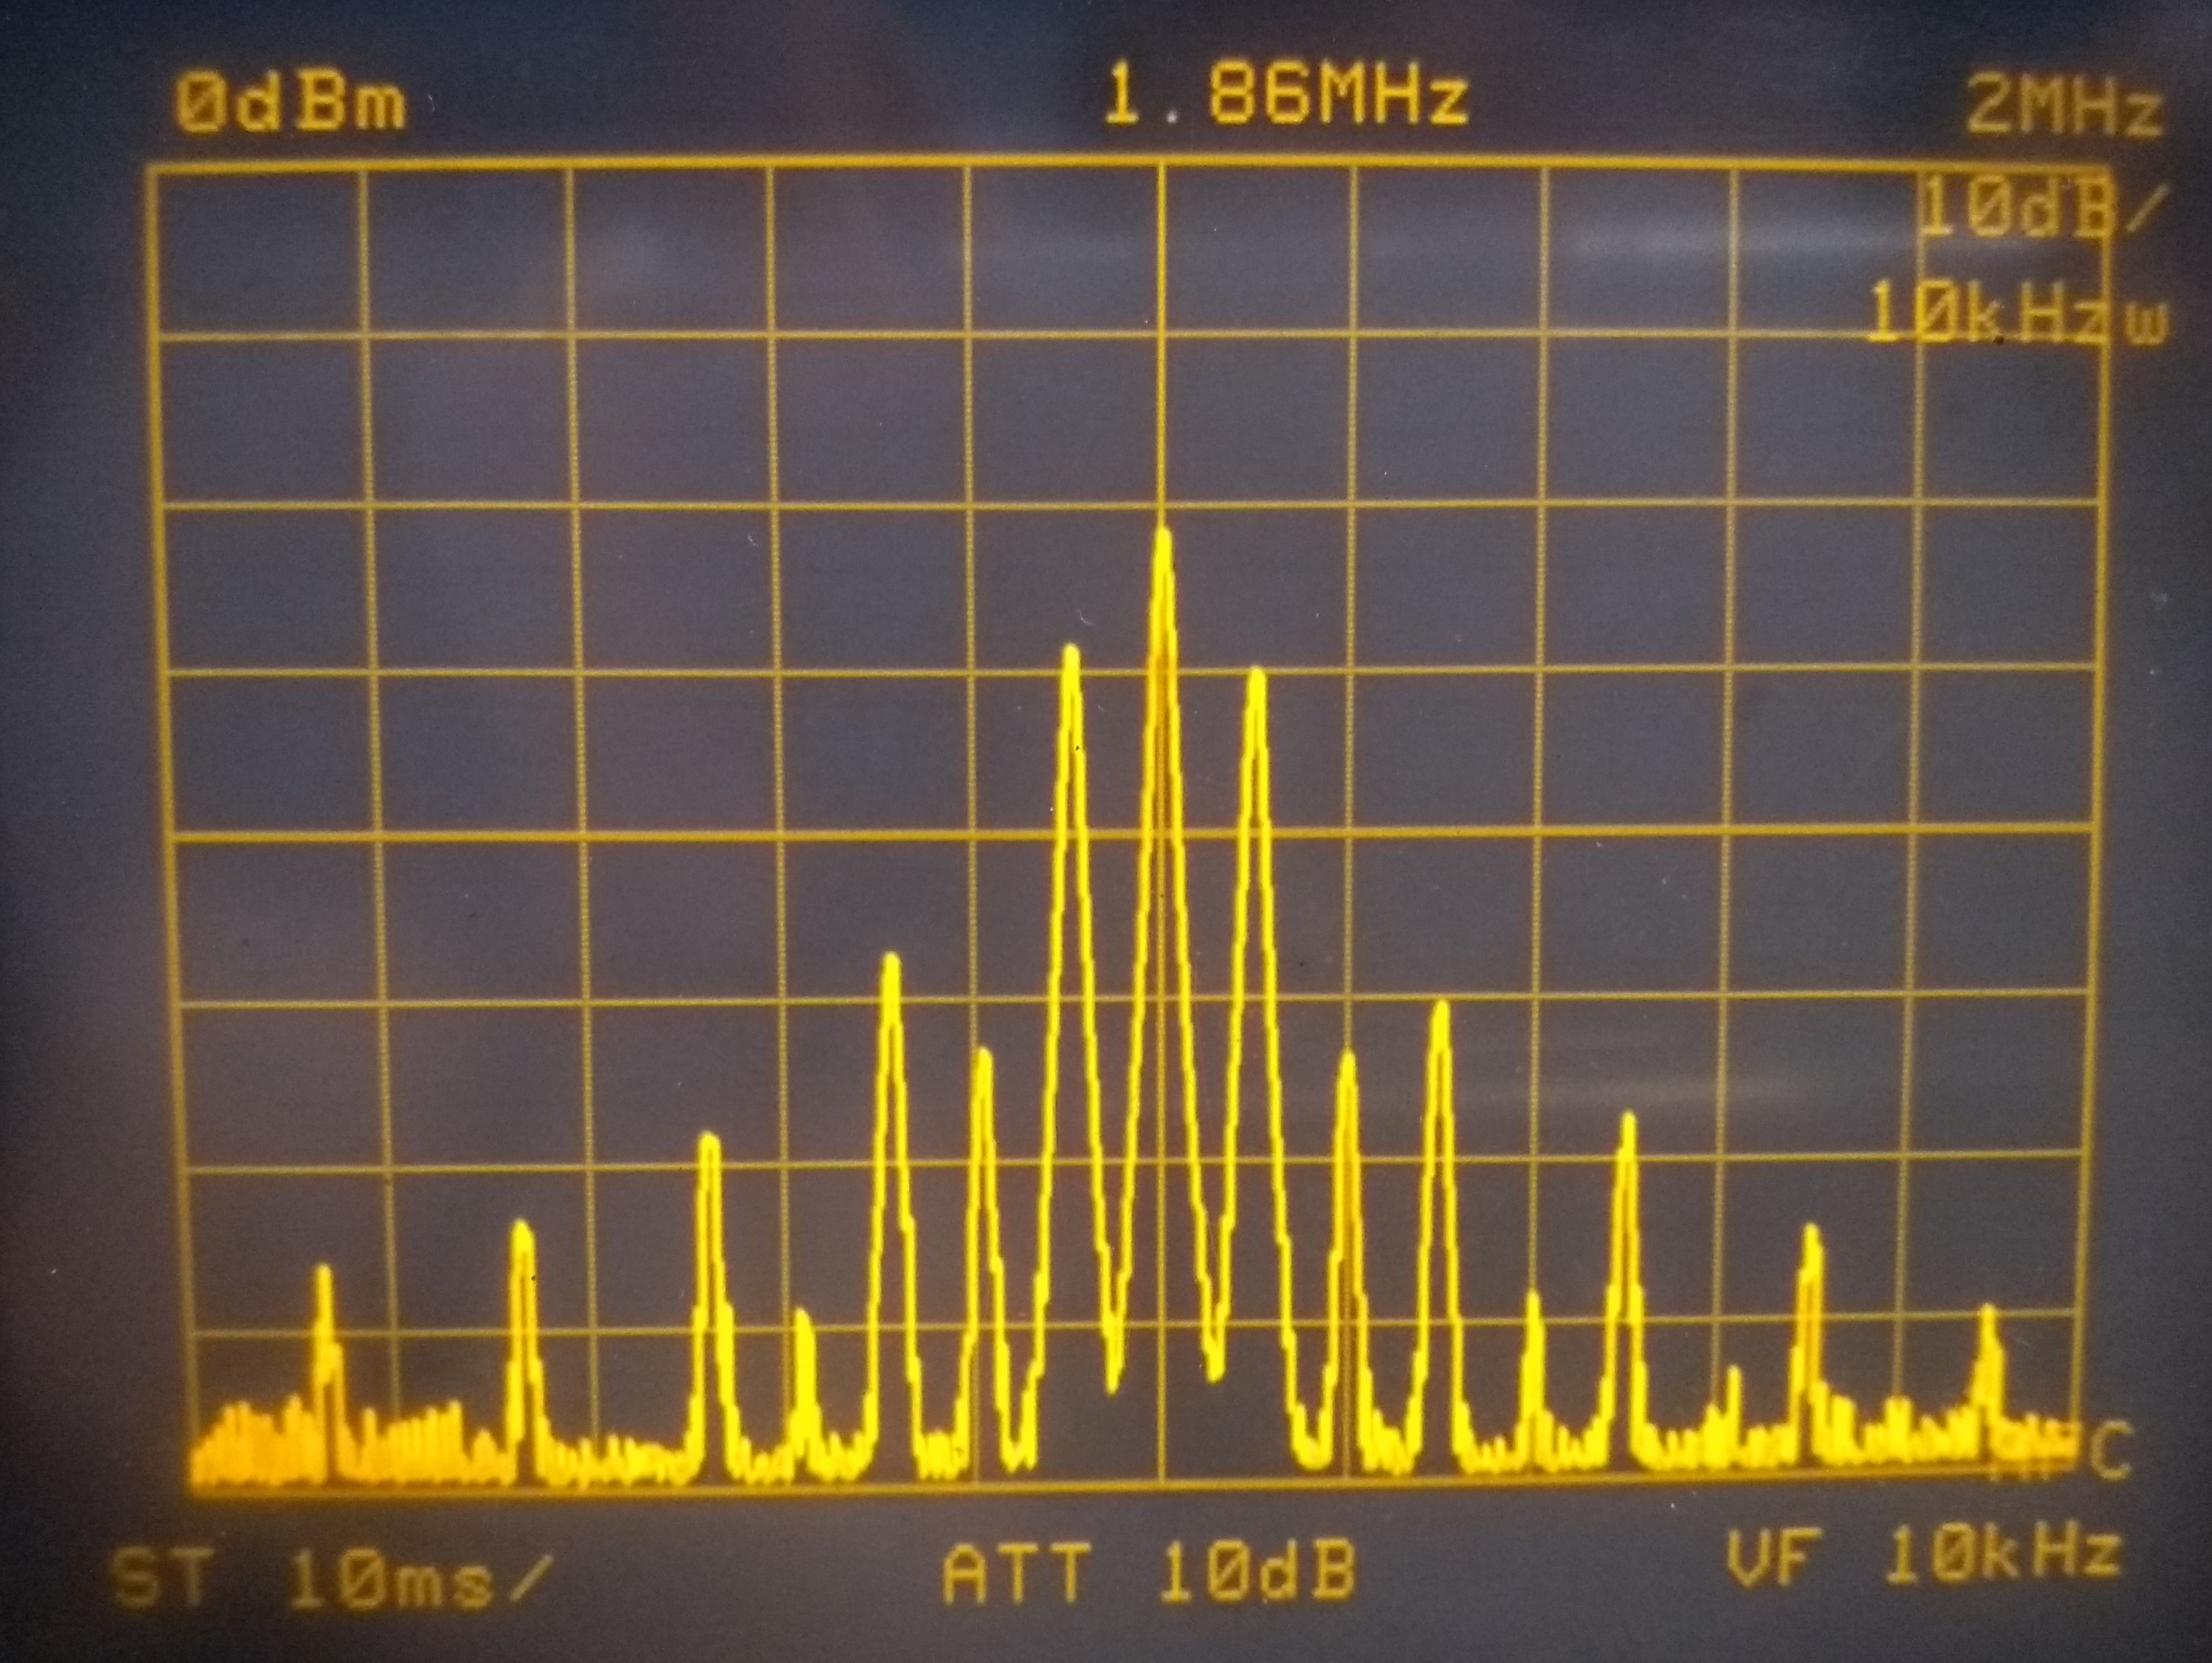
\includegraphics[scale=0.05]{imagenes/labo_tp5_ej3_c_1.jpg}
	\caption{Mediciones del espectro de una señal moduladora senoidal con m=1}
	\label{fig:ej1_labo_tp5_ej3_c_1}
\end{figure}
\begin{figure}[H]	
	\centering
	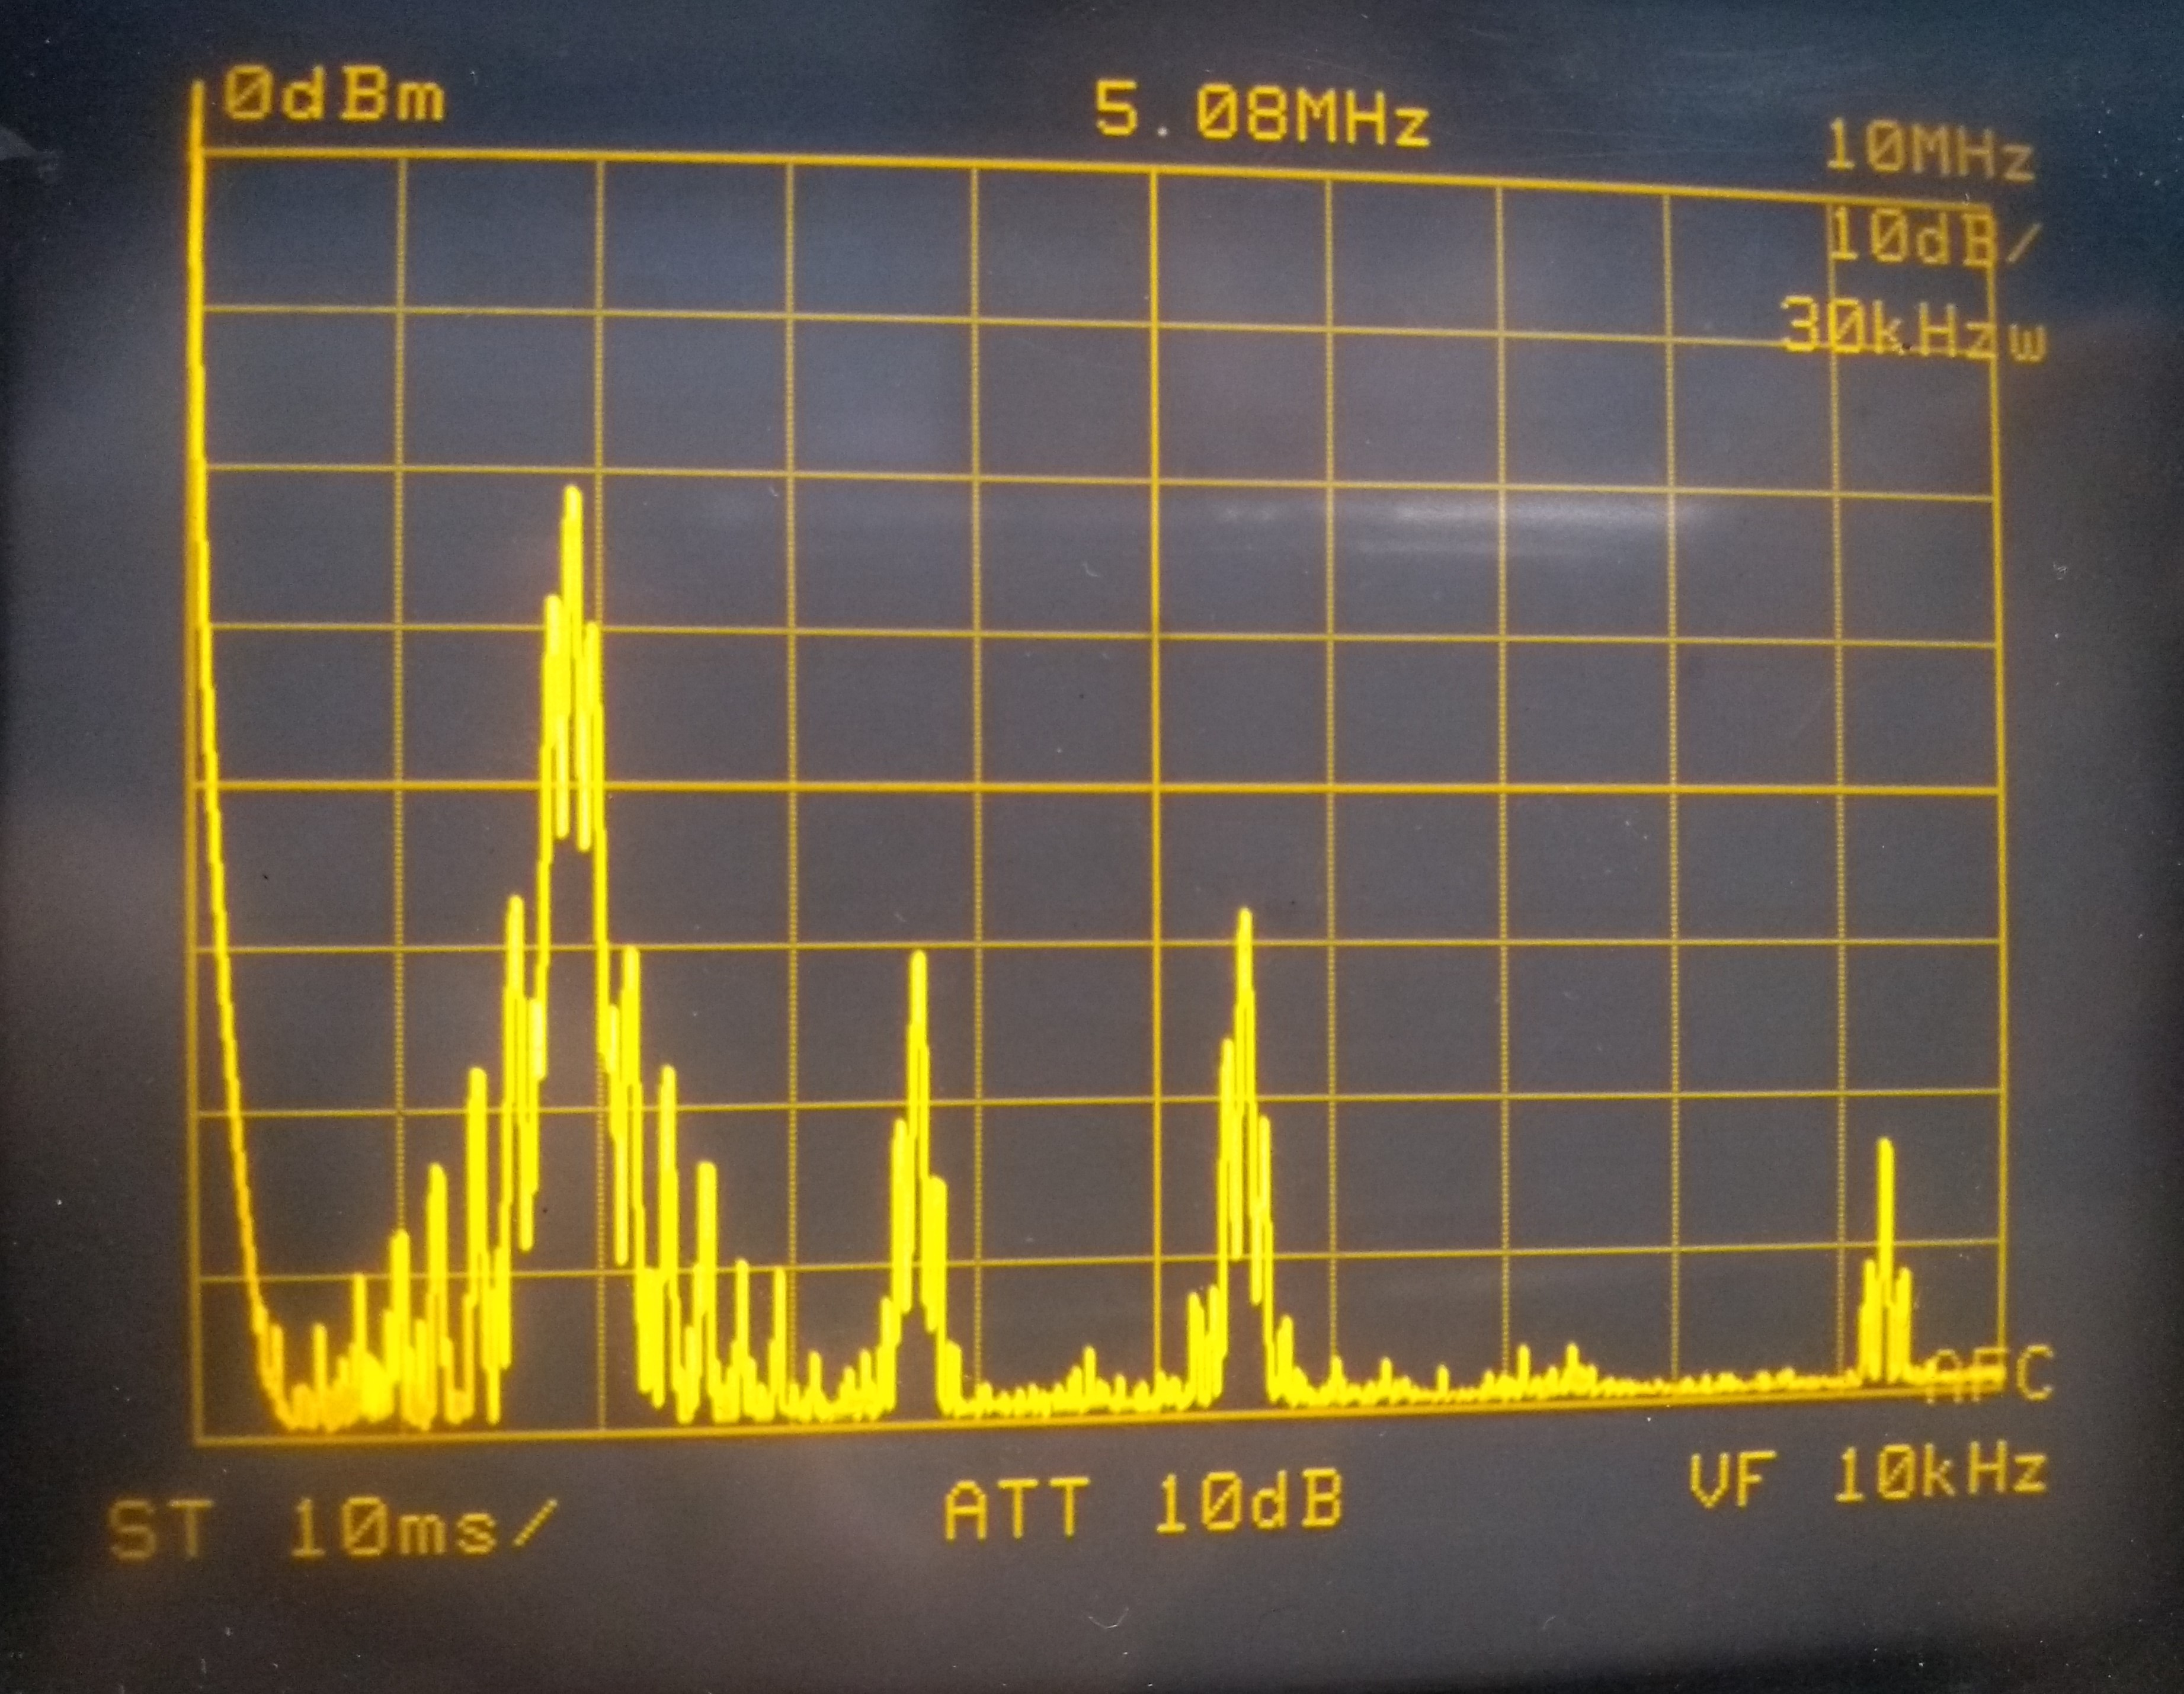
\includegraphics[scale=0.05]{imagenes/labo_tp5_ej3_c_2.jpg}
	\caption{Mediciones del espectro de una señal moduladora senoidal con m=1}
	\label{fig:ej1_labo_tp5_ej3_c_2}
\end{figure}
\begin{figure}[H]	
	\centering
	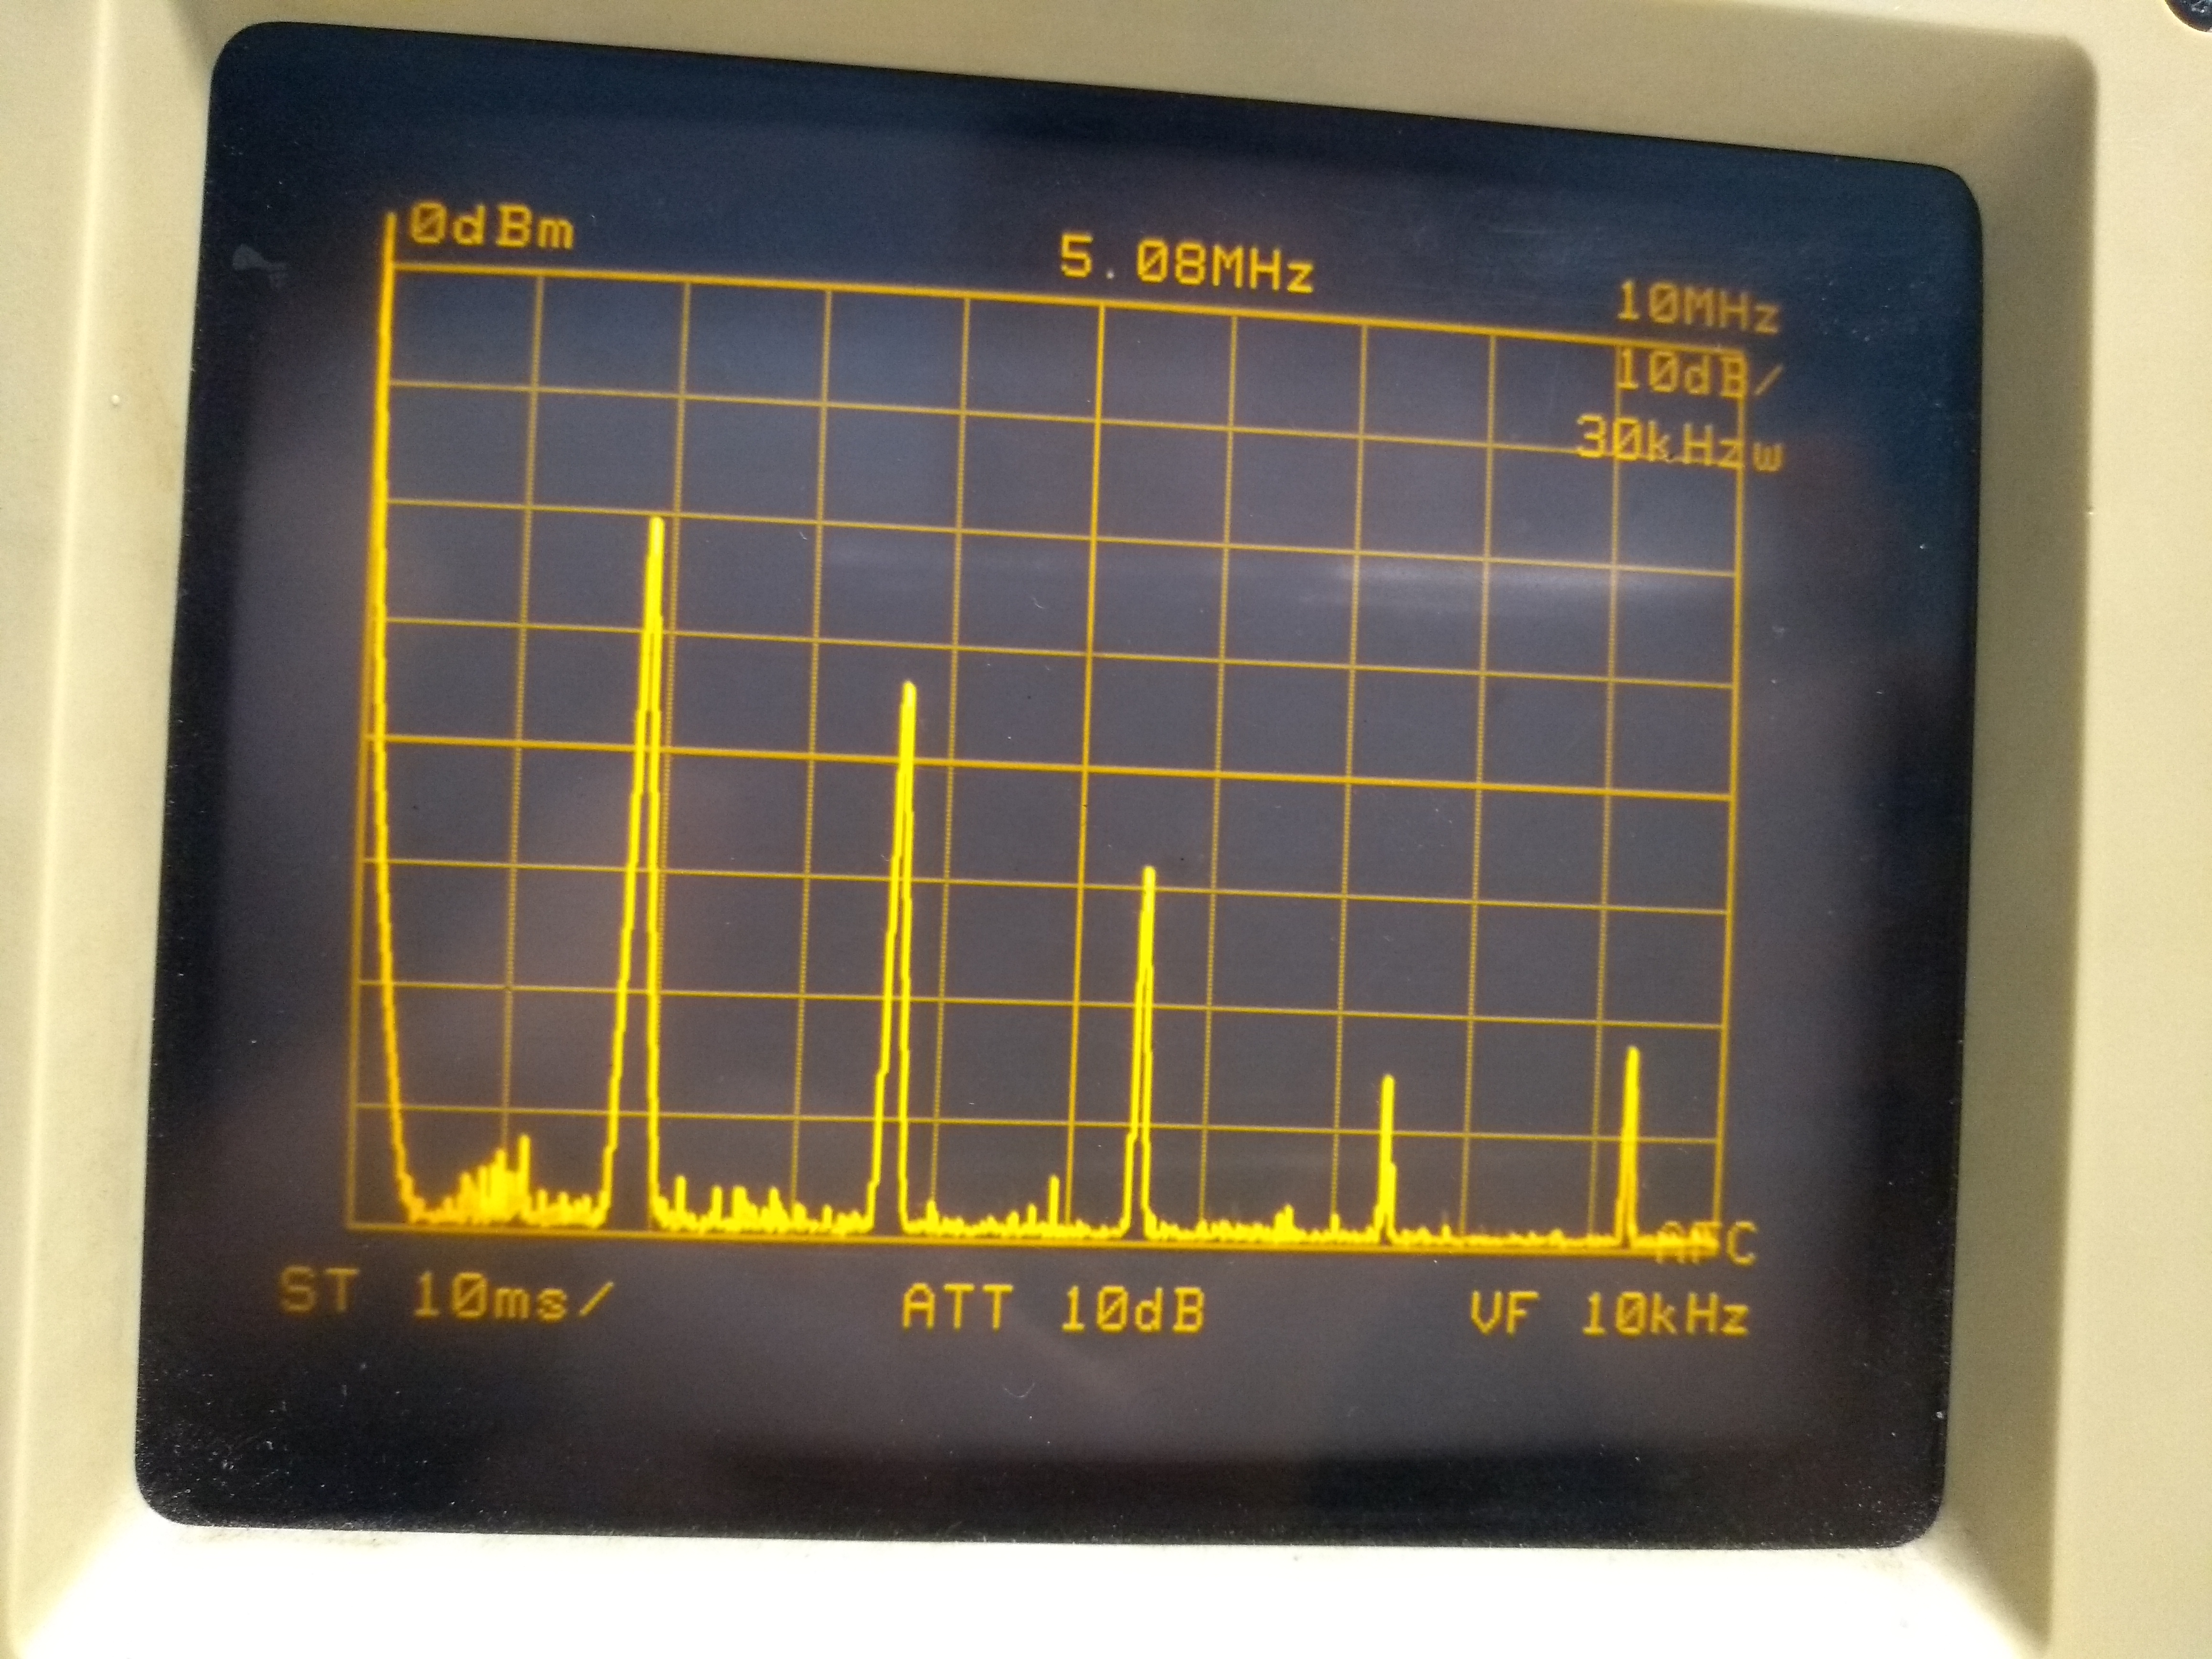
\includegraphics[scale=0.05]{imagenes/labo_tp5_ej3_d.jpg}
	\caption{Mediciones del espectro de una señal moduladora senoidal con m=1}
	\label{fig:ej1_labo_tp5_ej3_d}
\end{figure}

\end{document}
